\PassOptionsToPackage{unicode}{hyperref}
\documentclass[aspectratio=1610, captions=tableheading, 11pt]{beamer}
\usepackage{booktabs}
% Load packages you need here
\usepackage{polyglossia}
\setmainlanguage{german}

\usepackage{csquotes}
    
\usepackage{appendixnumberbeamer} 

\usepackage{caption}
\usepackage{varwidth}
\DeclareCaptionFormat{myformat}{%
  % #1: label (e.g. "Table 1")
  % #2: separator (e.g. ": ")
  % #3: caption text
  \begin{varwidth}{\linewidth}%
    \centering
    #1#2#3%
  \end{varwidth}%
}

\AtBeginSection[]{
  \begin{frame}
  \vfill
  \centering
  \begin{beamercolorbox}[sep=8pt,center,shadow=true,rounded=true]{title}
    \usebeamerfont{title}\insertsectionhead\par%
  \end{beamercolorbox}
  \vfill
  \end{frame}
}

\usepackage{amsmath}
\usepackage{amssymb}
\usepackage{mathtools}
\usepackage[mathrm=sym]{unicode-math}
\usepackage{relsize}
\usepackage{listings}

\usepackage[
  locale=DE,                 % deutsche Einstellungen
  separate-uncertainty=true, % immer Fehler mit \pm
  per-mode=reciprocal,       % ^-1 für inverse Einheiten
  % alternativ:
  % per-mode=reciprocal, % m s^{-1}
  % decimal-marker=., % . statt , f�r Dezimalzahlen
]{siunitx}

\usepackage{hyperref}
\usepackage{bookmark}
\usepackage[utf8]{inputenc}

% load the theme after all packages

\usetheme[
  showtotalframes, % show total number of frames in the footline
]{tudo}

% Put settings here, like
\unimathsetup{
  math-style=ISO,
  bold-style=ISO,
  nabla=upright,
  partial=upright,
  mathrm=sym,
}

\usepackage{tikz-feynman}
\usepackage{xfrac}
\usepackage{tikz}
\usetikzlibrary{shapes,arrows}

\tikzstyle{decision} = [rectangle, draw, fill=tucitron!20, 
    text width=15em, text centered, rounded corners, minimum height=2em]
\tikzstyle{onlytext} = [rectangle, draw=none, 
    text width=15em, text centered, rounded corners, minimum height=2em]
\tikzstyle{block} = [rectangle, draw, fill=tugreen!20, 
    text width=20em, text centered, rounded corners, minimum height=2em]
 \tikzstyle{blockH} = [rectangle, draw, fill=tugreen, 
    text width=20em, text centered, rounded corners, minimum height=2em]
\tikzstyle{smallblock} = [rectangle, draw, fill=tugreen!20, 
    text width=14em, text centered, rounded corners, minimum height=2em]
\tikzstyle{smallblockH} = [rectangle, draw, fill=tugreen, 
    text width=14em, text centered, rounded corners, minimum height=2em]
\tikzstyle{line} = [draw, -latex']
\tikzstyle{cloud} = [draw, ellipse,fill=red!20, node distance=3cm,
    minimum height=2em]
\tikzstyle{blocksmall} = [rectangle, draw, fill=tugreen!20, 
    text width=10em, text centered, rounded corners, minimum height=2em]

\setbeamertemplate{caption}{\raggedright\insertcaption\par}

% nur wenn akkurat auf dem Rechner installiert ist:
\setsansfont{Akkurat Light Office}[
  BoldFont=Akkurat Office Bold,
]


\author[jean-marco.alameddine@udo.edu]{Jean-Marco Alameddine}
\title{Particle propagation for CORSIKA in PROPOSAL}      
\date[19.06.2019]{19.06.2019}

\institute[%
  {
\includegraphics[height=0.9\headerheight]{e5b.pdf}}%
]{Technische Universität Dortmund}

\newcommand\CC{C\nolinebreak[4]\hspace{-.05em}\raisebox{.4ex}{\relsize{-3}{\textbf{++}}}\:}
%\titlegraphic{\includegraphics[height=0.4\textheight]{example-image-a}}

\usepackage{color}
\newcommand{\Hilight}{\makebox[0pt][l]{\color{tugreen}\rule[-4pt]{0.65\linewidth}{14pt}}}

\begin{document}



%%% TITLE

\begin{frame}
  \maketitle
\end{frame}

%%% Introduction %%%

\begin{frame}{Introduction}
  \begin{columns}
    \column{0.62\textwidth}
    \begin{center}
      \begin{itemize}
        \setlength\itemsep{0.5em}
        \item \textbf{PROPOSAL}: Tool to propagate particles through media
        \begin{itemize}
          \item[$\rightarrow$] MC simulations, multivariate statistics
        \end{itemize}
        \item \textbf{Requirements:} Accuracy, performance
        \item \textbf{Processes:} Energy losses, scattering, decays
        \item \CC library with Python bindings
      \end{itemize}
  \end{center}
  \column{0.35\textwidth}
      \begin{figure}
          \centering
          
\includegraphics[width=0.8\linewidth]{plots/github.pdf}
           \captionsetup{format=myformat}
          \caption*{https://github.com/tudo-astroparticlephysics/PROPOSAL}
      \end{figure}
  \end{columns}

\end{frame}

\begin{frame}{}
\begin{center}
\begin{tikzpicture}[node distance = 2.0cm, auto]
    % Place nodes
    \centering
    \node [blocksmall] (one) {MMC};
    \node [blocksmall, below of=one] (two) {PROPOSAL v1};
    \node [blocksmall, below of=two] (three) {PROPOSAL v2};
    \node [onlytext, right of=one, node distance=6cm] (repeat1) {JAVA};
    \node [onlytext, right of=two, node distance=6cm] (repeat2) {\CC};
    \node [onlytext, right of=three, node distance=6cm] (repeat3) {modern \CC, Polymorphism, \ldots};

    % Draw edges
    \path [line] (one) -- (two);
    \path [line] (two) -- (three);


\end{tikzpicture}
\end{center}
\end{frame}

\section{PROPOSAL code structure} 




\begin{frame}[fragile]
\begin{lstlisting}[language=C++,basicstyle=\ttfamily,keywordstyle=\color{red}, escapechar=\!]
Propagator(const ParticleDef&,
	   const std::vector<Sector::Definition>&,
	   const Geometry&,
	   const InterpolationDef&)
\end{lstlisting}
	\textcolor{tugreen}{\rule{\textwidth}{1pt}}\\%
	%\vspace*{-10px}
    \begin{itemize}
      \setlength\itemsep{0.5em}
      \item \texttt{Propagator} as base class to propagate a particle 
      \item Objects owns all information necessary for propagation

    \end{itemize}
\end{frame}



\begin{frame}[fragile]
\begin{lstlisting}[language=C++,basicstyle=\ttfamily,keywordstyle=\color{red}, escapechar=\!]
Propagator(!\Hilight!const ParticleDef&,
	   const std::vector<Sector::Definition>&,
	   const Geometry&,
	   const InterpolationDef&)
\end{lstlisting}
	\textcolor{tugreen}{\rule{\textwidth}{1pt}}\\%
    \begin{itemize}
      \setlength\itemsep{0.5em}
      \item \texttt{ParticleDef} includes static information about particle
      \item [$\rightarrow$] Wide range of predefined particles available 
      \item [$\rightarrow$] Modular structure: Simple creation of additional particles:
    \end{itemize}
\begin{lstlisting}[language=C++,basicstyle=\ttfamily,keywordstyle=\color{red}, escapechar=\!]
    ParticleDef new_mu = ParticleDef::Builder().SetMass(1000).build();
\end{lstlisting}
\end{frame}


\begin{frame}[fragile]
\begin{lstlisting}[language=C++,basicstyle=\ttfamily,keywordstyle=\color{red}, escapechar=\!]
Propagator(const ParticleDef&,
	   !\Hilight!const std::vector<Sector::Definition>&,
	   const Geometry&,
	   const InterpolationDef&)
\end{lstlisting}
	\textcolor{tugreen}{\rule{\textwidth}{1pt}}\\%
    \begin{itemize}
      \setlength\itemsep{0.5em}
      \item List of \texttt{Sector::Defintion} objects
      \item [$\rightarrow$] \emph{Chain of resposibility}: Propagation of our particle through several sectors
      \item [$\rightarrow$] Each \texttt{Sector} object is responsible for the propagation within its borders
    \end{itemize}
\end{frame}

\begin{frame}[fragile]
\begin{table}[htpb]
  \centering
  \begin{tabular}{lp{10cm}}
    \toprule
    Parameter & Description \\
    \midrule
    \texttt{Medium} & Medium of the sector \\
    \texttt{EnergyCutsSettings} & Stores $e_\text{cut}$ and $v_\text{cut}$ \\
    \texttt{Geometry} & Geometry of the sector \\
    \texttt{stopping\_decay} & Whether to force a final decay of the particle if its energy is $\leq e_\text{cut}$ \\
    \texttt{cont\_rand} & Whether to use continuous randomization \\
    \texttt{exact\_time} & Whether to calculate the time exactly out of the tracking integral or to use an approximation\\
    \texttt{scattering\_model} & Choice of the multiple scattering model\\
    \texttt{particle\_location} & Location of the particle \\
    \texttt{utility\_def} & Definition of cross section parameters \\
    \bottomrule
  \end{tabular}
  \label{tab:sector_def}
\end{table}
\texttt{Sector::Defintion} properties, adapted from \href{https://arxiv.org/abs/1809.07740}{arXiv:1809.07740}
\end{frame}


\begin{frame}[fragile]
\begin{lstlisting}[language=C++,basicstyle=\ttfamily,keywordstyle=\color{red}, escapechar=\!]
Propagator(const ParticleDef&,
	   const std::vector<Sector::Definition>&,
	   !\Hilight!const Geometry&,
	   const InterpolationDef&)
\end{lstlisting}
	\textcolor{tugreen}{\rule{\textwidth}{1pt}}\\%
    \begin{itemize}
      \setlength\itemsep{0.5em}
      \item Geometry describing the detector
    \end{itemize}
\end{frame}

\begin{frame}[fragile]
\begin{lstlisting}[language=C++,basicstyle=\ttfamily,keywordstyle=\color{red}, escapechar=\!]
Propagator(const ParticleDef&,
	   const std::vector<Sector::Definition>&,
	   const Geometry&,
	   !\Hilight!const InterpolationDef&)
\end{lstlisting}
	\textcolor{tugreen}{\rule{\textwidth}{1pt}}\\%
    \begin{itemize}
      \setlength\itemsep{0.5em}
      \item \texttt{InterpolationDef} as an optional parameter
      \item [$\rightarrow$] When used, calculated crosssections are saved in interpolation tables
      \item [$\rightarrow$] Error of interpolation compared to integration: $\leq \num{e-5}$
      \item [$\rightarrow$] Performance increased by several orders of magnitude
    \end{itemize}
\end{frame}

\begin{frame}[fragile]
\begin{lstlisting}[language=C++,basicstyle=\ttfamily,keywordstyle=\color{red}, escapechar=\!]
Propagator::Propagator(const ParticleDef& particle_def, 
                       const std::string& config_file)
\end{lstlisting}
	\textcolor{tugreen}{\rule{\textwidth}{1pt}}\\%
    \begin{itemize}
      \setlength\itemsep{0.5em}
      \item Simple usage of a configuration (json) file is possible
    \end{itemize}
\end{frame}

\begin{frame}
\begin{figure}
    \centering
    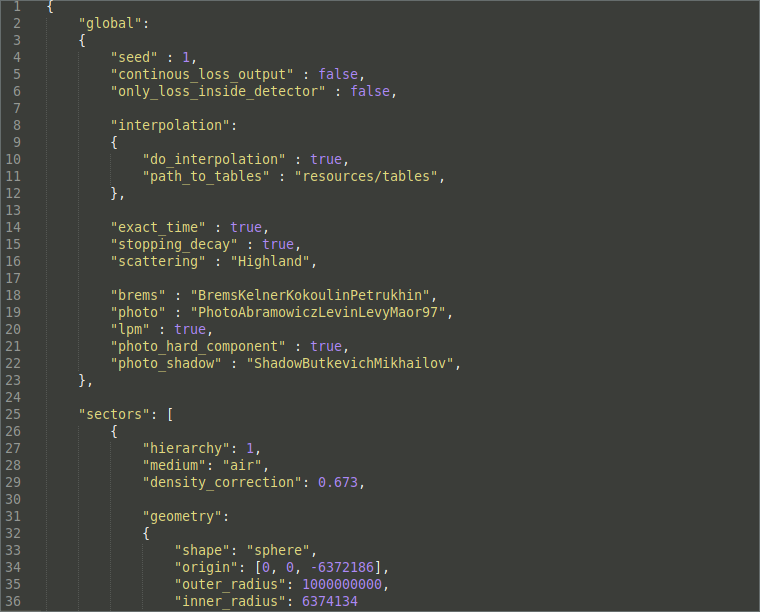
\includegraphics[height=0.99\textheight]{plots/config.png}
    %\caption*{Propagation of $\num{e4}$ muons with energy $\SI{e8}{\mega\electronvolt}$ through $\SI{300}{\metre}$ of standard rock.}
    \label{fig:1}
\end{figure}
\end{frame}

\section{Propagation algorithm}

\begin{frame}[fragile]
\begin{lstlisting}[language=C++,basicstyle=\ttfamily,keywordstyle=\color{red}, escapechar=\!]
std::vector<DynamicData*> Propagator::Propagate(double MaxDistance_cm)
\end{lstlisting}
	\textcolor{tugreen}{\rule{\textwidth}{1pt}}\\%
	\vspace*{10px}
	\begin{tikzpicture}[node distance = 2.4cm, auto]
    % Place nodes
    \node [block] (one) {Choose next \texttt{Sector}};
    \node [block, below of=one] (two) {Propagate in chosen \texttt{Sector} until \texttt{MaxDistance} reached or sector border reached };
    \draw [->] (one) -- node[name=u] {} (two);

    \node [decision, right of=u, node distance=7.5cm] (repeat) {Particle did not reach \texttt{MaxDistance}, did not decay, energy not below $e_\text{low}$};

    % Draw edges

    \path [line, dashed] (two) -| (repeat);
    \path [line, dashed] (repeat) |- (one);
	\end{tikzpicture}

\end{frame}


\begin{frame}[fragile]
\begin{lstlisting}[language=C++,basicstyle=\ttfamily,keywordstyle=\color{red}, escapechar=\!]
double Sector::Propagate(double distance)
\end{lstlisting}
	\textcolor{tugreen}{\rule{\textwidth}{1pt}}\\%
	\vspace*{10px}
	\textbf{Remember:} Differentiate between continuous losses and stochastic losses !
	\vspace*{-20px}
	\begin{center}

 		\huge
 		\begin{align*}
 		    \underset{\text{continuous losses}}{v < v_\text{cut}} &&  \underset{\text{stochastic losses}}{v > v_\text{cut}}
 		\end{align*}\\
 		\vspace{20px}
 		\centering
 		  \Large
 		with $v_\text{cut} = \text{min}\left[\sfrac{e_\text{cut}}{E}, v\prime_\text{cut} \right]$

	\end{center}

\end{frame}


\begin{frame}[fragile]
\begin{lstlisting}[language=C++,basicstyle=\ttfamily,keywordstyle=\color{red}, escapechar=\!]
double Sector::Propagate(double distance)
\end{lstlisting}
	\textcolor{tugreen}{\rule{\textwidth}{1pt}}\\%
	\vspace*{10px}
	\textbf{Remember:} Differentiate between continuous losses and stochastic losses !
	\begin{center}
	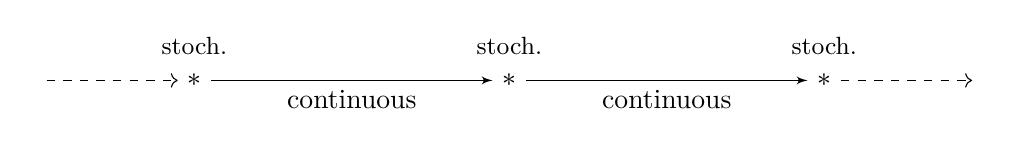
\begin{tikzpicture}[node distance=2cm]

	% nodes
	\node (A) at (2, 0) {};
	\node[label={\small \text{stoch.}}] (B) at (4, 0) {$*$};
	\node[label={\small \text{stoch.}}] (C) at (8, 0) {$*$};
	\node[label={\small \text{stoch.}}] (D) at (12, 0) {$*$};
	\node (E) at (14, 0) {};

	
	% arrows
	\draw [dashed,->] (A) -- node[below] {} (B);
	\draw [line] (B) -- node[below] {\text{continuous}} (C);
	\draw [line] (C) -- node[below] {\text{continuous}} (D);
	\draw [dashed,->] (D) -- node[below] {} (E);

	
	\end{tikzpicture}
	\end{center}

\end{frame}

\begin{frame}[fragile]

	\begin{tikzpicture}[node distance = 1.8cm, auto]
    % Place nodes
    \node [block] (one) {Sample energy when next interaction occurs (stochastic loss or decay)};
    \onslide<2>{\node [blockH] (one) {Sample energy when next interaction occurs (stochastic loss or decay)};}

    \node [block, below of=one] (two) {Calculate displacement until next interaction};
    \onslide<3>{\node [blockH, below of=one] (two) {Calculate displacement until next interaction};}

    \draw [line] (two) -- node[name=u] {} (three);
    \node [block, below of=two] (three) {Sample scattering};
    \onslide<5>{\node [blockH, below of=two] (three) {Sample scattering};}
    \node [block, below of=three] (four) {Continuous randomization};
    \onslide<6>{\node [blockH, below of=three] (four) {Continuous randomization};}

    \node [smallblock, right of=u, node distance=7.5cm] (repeat) {Calculate final energy\\ until sector border};
    \onslide<4>{\node [smallblockH, right of=u, node distance=7.5cm] (repeat) {Calculate final energy\\ until sector border};}

    % Draw edges
    \path [line] (one) -- (two);
    \path [line] (two) -| node[above] {\text{displacement overshoots border limit}} (repeat);
    \path [line] (repeat) |- (three);
    \path [line] (two) -- (three);
    \path [line] (three) -- (four);

	\end{tikzpicture}

\end{frame}

\begin{frame}
\begin{figure}
    \centering
    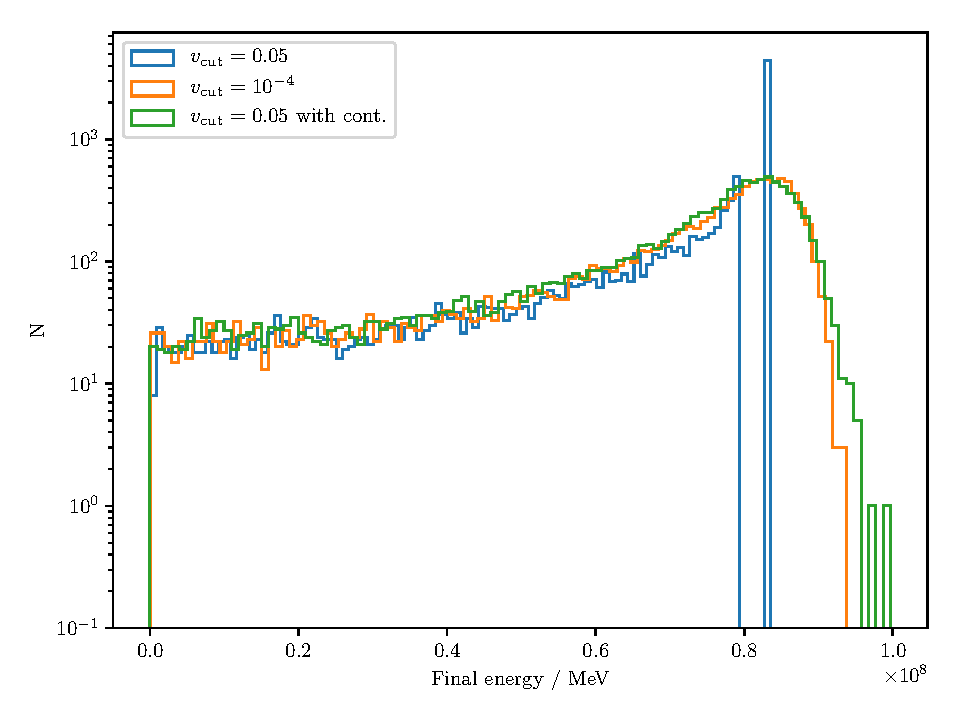
\includegraphics[height=0.85\textheight, trim=0.5cm 0.2cm 0.5cm 0.5cm,clip=true]{plots/mu_continuous_new.pdf}
    \caption*{Propagation of $\num{e4}$ muons with energy $\SI{e8}{\mega\electronvolt}$ through $\SI{300}{\metre}$ of standard rock.}
    \label{fig:1}
\end{figure}
\end{frame}


\begin{frame}[fragile]

	\begin{tikzpicture}[node distance = 1.8cm, auto]
    % Place nodes
    \node [block] (one) {Continuous randomization};

    \node [smallblock, below of=one] (two) {Sample type of stochastic loss};
    \onslide<3>{\node [smallblockH, below of=one] (two) {Sample type of stochastic loss};}


    \node [smallblock, right of=two, node distance=7.5cm] (three) {Sample decay};
    \onslide<2>{\node [smallblockH, right of=two, node distance=7.5cm] (three) {Sample decay};}


    \node [smallblock, below of=two] (four) {Sample energy loss};
    \onslide<4>{\node [smallblockH, below of=two] (four) {Sample energy loss};}

    \node [block, below of=four] (five) {Repeat algorithm if $E > e_\text{low}$ and particle has not decayed};
    \onslide<5>{\node [blockH, below of=four] (five) {Repeat algorithm if $E > e_\text{low}$ and particle has not decayed};}

    % Draw edges
    \path [line] (one) -- (two);
    \path [line] (one) -| (three);
    \path [line] (three) |- (five);
    \path [line] (two) -- (four);
    \path [line] (four) -- (five);

	\end{tikzpicture}

\end{frame}


\begin{frame}[fragile]
\begin{lstlisting}[language=C++,basicstyle=\ttfamily,keywordstyle=\color{red}, escapechar=\!]
std::vector<DynamicData*> Propagator::Propagate(double MaxDistance_cm);
\end{lstlisting}
	\textcolor{tugreen}{\rule{\textwidth}{1pt}}\\%
	\vspace*{10px}
	\textbf{Return value:} List of \texttt{DynamicData} objects, including
	\begin{enumerate}
		\item Stochastic losses (type, energy, position, time, \ldots)
		\item Decay particles
		\item Produced particles
		\item (Continuous losses)
	\end{enumerate}
\end{frame}

\begin{frame}[fragile]
  \vspace{-10mm}
\begin{lstlisting}[language=C++,basicstyle=\ttfamily,keywordstyle=\color{red}, escapechar=\!]
Propagator prop(MuMinusDef::Get(), "resources/config.json");
Particle& mu = prop.GetParticle();
Particle mu_backup(mu);

mu_backup.SetEnergy(9e6); //energy in MeV
mu_backup.SetDirection(Vector3D(0, 0, -1));

std::vector<double> ranges;

for (int i = 0; i < 10; i++){
    mu.InjectState(mu_backup);
    prop.Propagate();  
    ranges.push_back(mu.GetPropagatedDistance());
}
// ...
\end{lstlisting}
\end{frame}

\begin{frame}[fragile]
  \vspace{-10mm}
\begin{lstlisting}[language=python,basicstyle=\ttfamily,keywordstyle=\color{red}, escapechar=\!]
prop = pp.Propagator(particle_def=pp.particle.MuMinusDef.get(), 
		     config_file="path/to/config.json")
mu = prop.particle
mu_backup = pp.particle.Particle(mu)

mu_backup.energy = 9e6 #energy in MeV
mu_backup.direction = pp.Vector3D(0, 0, -1)

ranges = []

for i in range(10):
    mu.inject_state(mu_backup)
    secondaries = prop.propagate()
    ranges.append(prop.particle.propagated_distance)
\end{lstlisting}

\end{frame}


\section{PROPOSAL changes for CORSIKA}

\begin{frame}{Displacement calculation}
	\vspace{-10mm}
	\begin{center}
		\begin{align*}
			-f\left(E\right) = \frac{\mathrm{d}E}{\mathrm{d}x}
		\end{align*}
	\end{center}
	\vspace{-5mm}
	\begin{columns}
		\column{0.5\textwidth}
			\begin{center}
			\textbf{Homogeneous medium:}
			\begin{align*}
				-f\left(E\right) {\color{red}{}\rho_0} &= \frac{\mathrm{d}E}{\mathrm{d}x}\\
				\mathrm{d}x &= -\frac{1}{{\color{red}{}\rho_0}} \frac{\mathrm{d}E}{f\left(E\right)}\\
				x_f &= x_i - \frac{1}{{\color{red}{}\rho_0}} \int_{E_i}^{E_f} \frac{\mathrm{d}E}{f\left(E\right)}
			\end{align*}
			\end{center}
		\column{0.5\textwidth}
			\begin{center}
			\textbf{Non-homogeneous medium}
			\begin{align*}
				-f\left(E\right) {\color{red}{}\rho\left(x\right)} &= \frac{\mathrm{d}E}{\mathrm{d}x}\\
				\mathrm{d}x {\color{red}{}\rho\left(x\right)} &= -\frac{\mathrm{d}E}{f\left(E\right)}\\
				\int_{x_f}^{x_i} \mathrm{d}x {\color{red}{}\rho\left(x\right)} &= -  \int_{E_i}^{E_f} \frac{\mathrm{d}E}{f\left(E\right)}
			\end{align*}
			\end{center}
	\end{columns}
		\begin{columns}
		\column{0.5\textwidth}

		\column{0.5\textwidth}
			\begin{center}
			solve for $x_f$
			\end{center}
	\end{columns}

\end{frame}

\begin{frame}[t]
  \vspace{-5mm}
  \begin{minipage}[t][0.8\textheight][t]{\textwidth}
      \begin{columns}
    \column{0.5\textwidth}
      \begin{figure}
          \centering
          
\includegraphics[width=0.6\linewidth]{plots/github.pdf}
           \captionsetup{format=myformat}
          \caption*{https://github.com/tudo-\\astroparticlephysics/PROPOSAL}
      \end{figure}
    \column{0.5\textwidth}
      \begin{figure}
          \centering
          
\includegraphics[width=0.6\linewidth]{plots/arxiv.pdf}
          \captionsetup{format=myformat}
          \caption*{https://arxiv.org/abs/1809.07740 \\ \phantom{astroparticlephysics/PROPOSAL}}
      \end{figure}
  \end{columns}
  \end{minipage}
  \vfill
  \begin{minipage}{\textwidth}
      \smaller
      \begin{center}
      PROPOSAL may be modified and distrubuted under terms of a modified LGPL license.\\More information on our GitHub page.
      \end{center}
  \end{minipage}
\end{frame}
\end{document}

\appendix
\section{Backup slides} 

%%% Muon pair prodction


\begin{frame}{Propagation}
  \Huge
  \begin{align*}
      \frac{\mathrm{d}\sigma}{\mathrm{d}v} \quad \underbrace{\longrightarrow}_{?} \quad \text{energy losses}
  \end{align*}
\end{frame}

\begin{frame}{Propagation}
  \huge
  \begin{align*}
      \underset{\text{continuous losses}}{v < v_\text{cut}} &&  \underset{\text{stochastic losses}}{v > v_\text{cut}}
  \end{align*}\\
  \vspace{20px}
  \centering
    \Large
  with $v_\text{cut} = \text{min}\left[\sfrac{e_\text{cut}}{E}, v\prime_\text{cut} \right]$
\end{frame}

\begin{frame}{Propagation}
\begin{tikzpicture}[node distance = 1.7cm, auto]
    % Place nodes
    \node [block] (one) {Calculate energy at which a stochastic loss occurs};
    %\node [block, below of=one] (two) {Calculate continuous losses via:\\ \vspace{5px}
 %$- \left\langle \frac{\mathrm{d}E}{\mathrm{d}x} \right\rangle \propto E \int_{v_\text{min}}^{v_\text{cut}} v \frac{\mathrm{d}\sigma}{\mathrm{d}v} \mathrm{d}v$};
    \node [block, below of=one] (two) {Calculate type of stochastic loss};
    \node [block, below of=two] (three) {Sample the stochastic energy loss via:\\\vspace{5px} $\frac{1}{\sigma} \int_{v_\text{cut}}^{v\left(\xi\right)} \frac{\mathrm{d}\sigma}{\mathrm{d}v} \mathrm{d}v = \xi$};
    \node [decision, right of=two, node distance=7.5cm] (repeat) {Repeat until $E < e_0$ or\\ particle reaches section border};

    % Draw edges
    \path [line] (one) -- (two);
    \path [line] (two) -- (three);
    %\path [line] (three) -- (four);
    \path [line, dashed] (three) -| (repeat);
    \path [line, dashed] (repeat) |- (one);



\end{tikzpicture}
\end{frame}

\begin{frame}
\begin{columns}
  \column{0.35\textwidth}
  \begin{center}
    \begin{minipage}{0.9\textwidth}
      \textbf{Standard interactions:}
      \begin{itemize}
        \item $e$ pair production
        \item Bremsstrahlung
        \item Photonuclear
        \item Ionization
      \end{itemize}
    \end{minipage}
  \end{center}

  \column{0.5\textwidth}
  \begin{center}
    \begin{minipage}{0.9\textwidth}
      \textbf{Rare interactions:}
      \begin{itemize}
         \item $\mu$ pair production
          \item Weak interaction
          \item[$\rightarrow$] Negligible contribution to overall energy loss
          \item[$\rightarrow$] Observable, interesting signature
      \end{itemize}
    \end{minipage}
  \end{center}

\end{columns}
\end{frame}





\begin{frame}

\begin{figure}
    \centering
    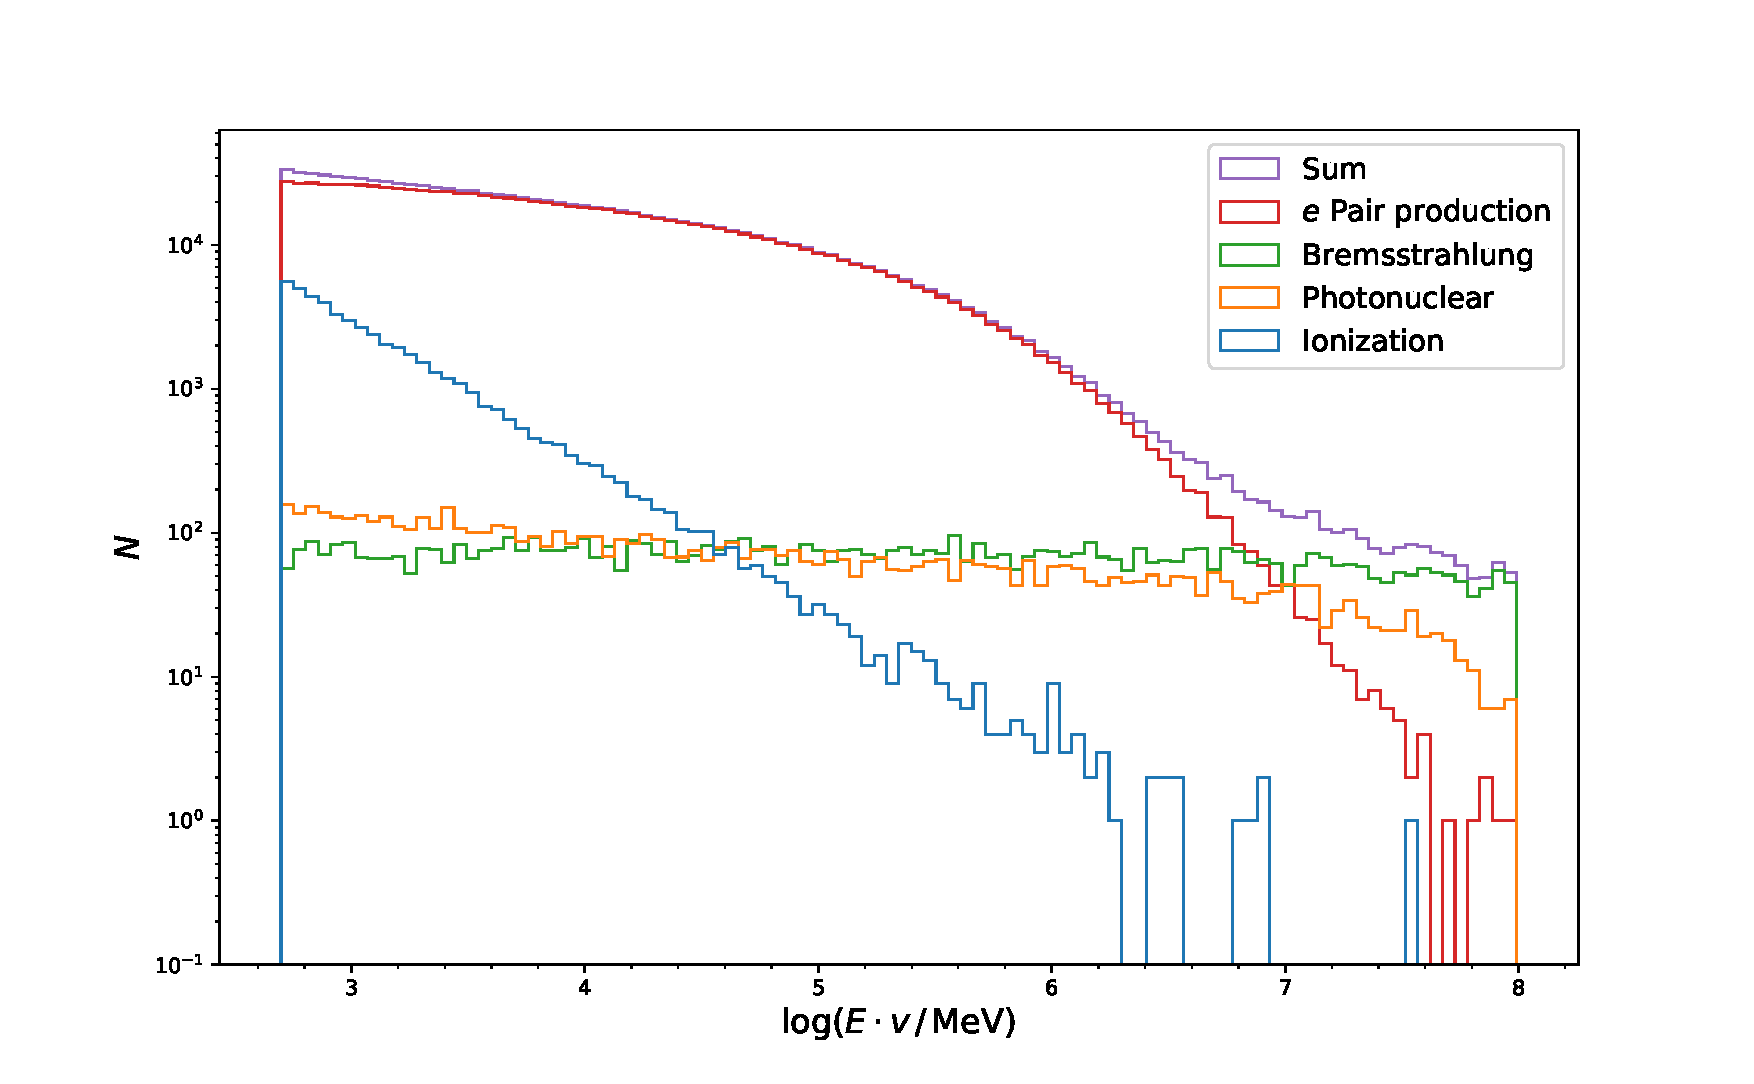
\includegraphics[height=0.85\textheight, trim=1.9cm 0.5cm 1.9cm 2cm,clip=true]{plots/standard.pdf}
    \caption*{Propagation of $\num{e4}$ muons with energy $\SI{e8}{\mega\electronvolt}$ through $\SI{100}{\metre}$ of standard rock.}
    \label{fig:1}
\end{figure}
\end{frame}

\begin{frame}<presentation:0>[noframenumbering]
\begin{figure}
  \begin{minipage}[c]{0.7\textwidth}
    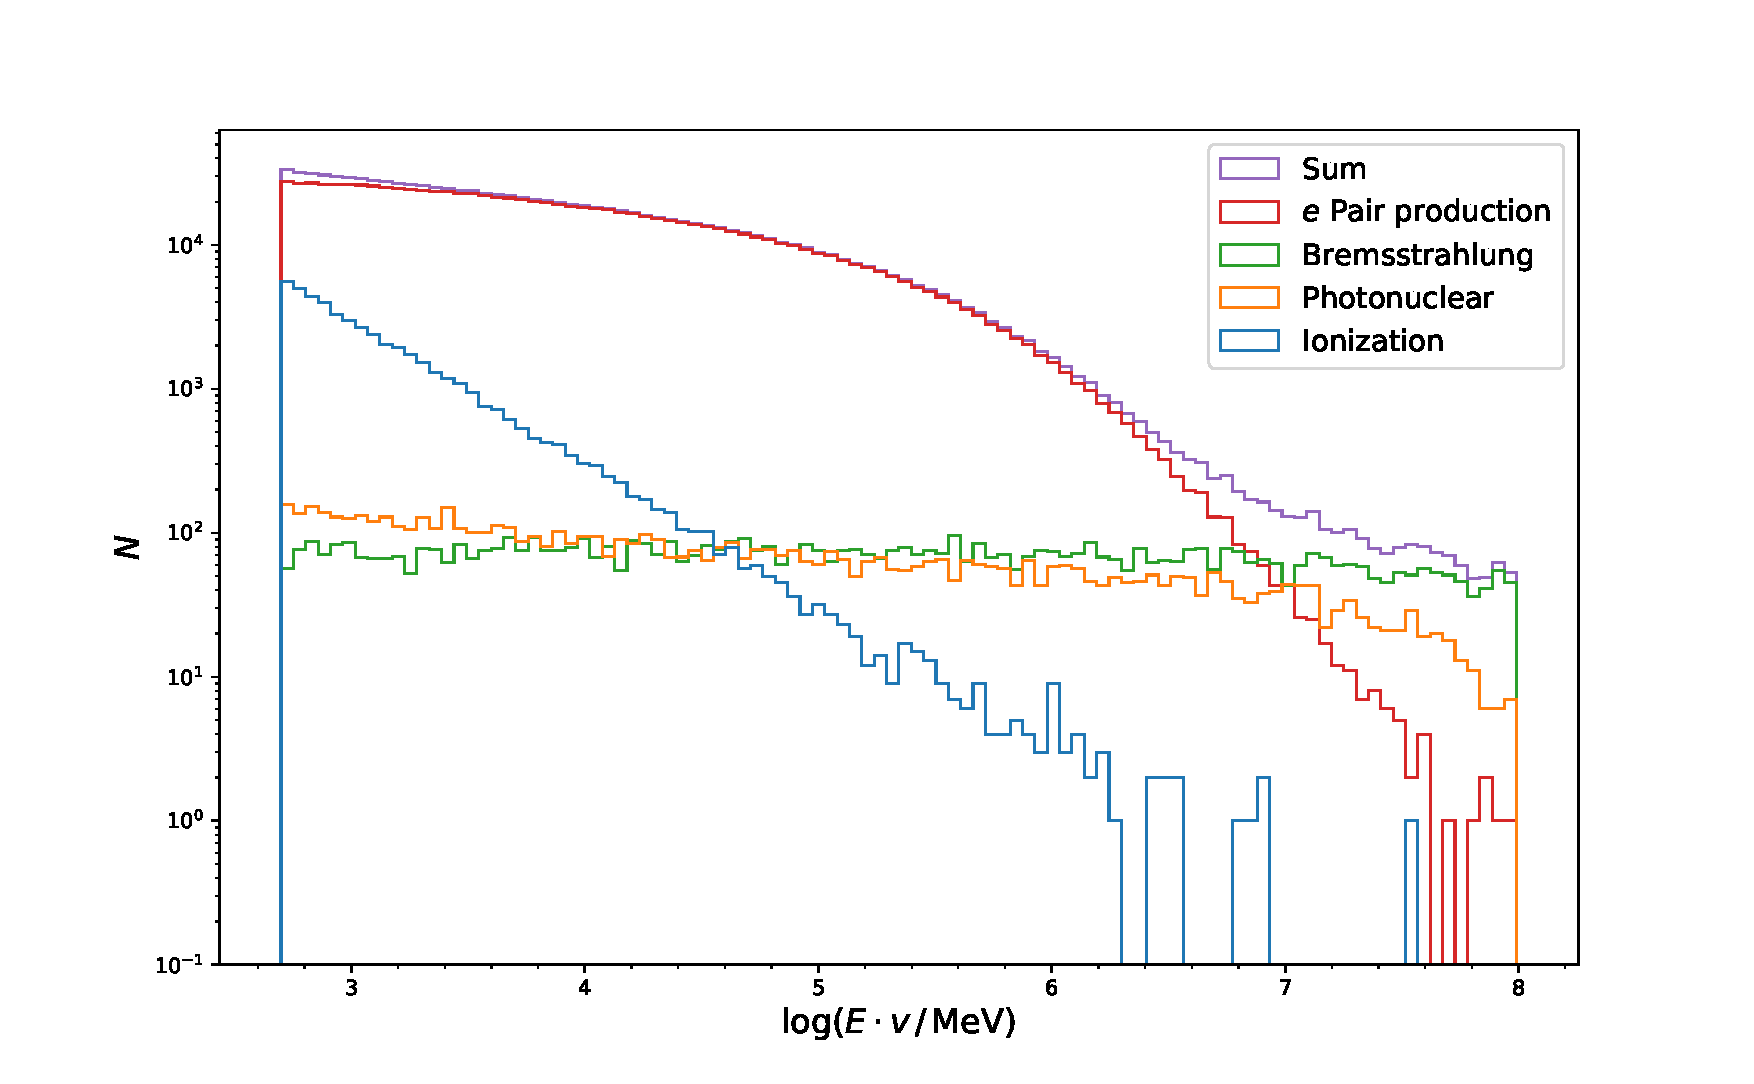
\includegraphics[width=\textwidth , trim=1.9cm 0.5cm 1.9cm 2cm,clip=true]{plots/standard.pdf}
  \end{minipage}\hfill
  \begin{minipage}[c]{0.3\textwidth}
    Propagation of $\num{e4}$ muons with energy $\SI{e8}{\mega\electronvolt}$ through $\SI{100}{\metre}$ of standard rock.
     \label{fig:03-03}
  \end{minipage}
\end{figure}

\end{frame}


\begin{frame}{Direct Production of Muon Pairs}
  \begin{columns}
    \column{0.5\textwidth}
    \begin{center}
      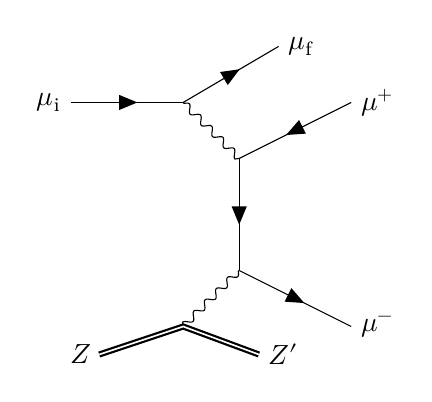
\begin{tikzpicture}
      \centering
       % Sizes
       \pgfmathsetmacro{\len}{0.05cm}
       \pgfmathsetmacro{\halflen}{\len/4}
       \pgfmathsetmacro{\vertexsize}{\len/20}
       \begin{feynman}
           % vertices
           \vertex (a) at (0, 0);
           \vertex (b) at (0, -1*\len);
           \vertex (d) at (-0.5*\len, 0.5*\len);
           \vertex (c) at (-0.5*\len, -1.5*\len);
           \vertex (i1) at (-1.5*\len, 0.5*\len);
           \vertex (i2) at (0, 1.5*\len);
           \vertex (f1) at (\len, 0.5*\len);
           \vertex (f2) at (\len, -1.5*\len);
           \vertex (f3) at (0.5, 1*\len);
           \vertex (z1) at (-1.25*\len, -1.75*\len);
           \vertex (z2) at (0.25, -1.75*\len);
     
           % draw diagram
           \diagram* {
             (i1) -- [fermion] (d) -- [fermion] (f3),
             (d) -- [boson] (a),
             (f1) -- [fermion] (a),
             (a) -- [fermion] (b),
             (b) -- [fermion] (f2),
             (b) -- [boson] (c),
           };
           \draw[thick, double] (z1) -- (c) -- (z2);
     
           % labels
           \node[left] at (i1) {$\mu_\text{i}$};
           \node[right] at (f3) {$\mu_\text{f}$};
           \node[right] at (f1) {$\mu^+$};
           \node[right] at (f2) {$\mu^-$};
           \node[left] at (z1) {$Z$};
           \node[right] at (z2) {$Z'$};
      \end{feynman}
    \end{tikzpicture}
  \end{center}
  \column{0.5\textwidth}
    Energy fraction transferred to the muon pair:
      \begin{align*}
        v = \frac{\left( \epsilon_+ + \epsilon_- \right)}{E} \\[0.1cm]
      \end{align*}
    Asymmetry parameter:
    \begin{align*}
      \rho = \frac{\left( \epsilon_+ - \epsilon_- \right)}{\left( \epsilon_+ + \epsilon_- \right)} \\[0.1cm]
    \end{align*}

    $E$: Initial energy of the incoming muon $\mu_\text{i}$ \\
    $\epsilon_\pm$: Energy of the produced (anti)muon

  \end{columns}

\end{frame}

%<presentation:0>[noframenumbering]
\begin{frame}{Double-differential cross section}

For production of muon pairs \footnote{Kelner, Kokoulin, Petrukhin: Phys. of Atomic Nuclei, Vol. 63, No. 9, 2000, pp. 1603-1611}:
\begin{align*}
  \frac{\mathrm{d}\sigma}{\mathrm{d}v \mathrm{d}\rho} &= \frac{2}{3\pi} (Z \alpha r_\mu)^2 \frac{1-v}{v} \Phi(v, \rho) \ln \left( X \right)
\intertext{%
For production of electron positron pairs \footnotemark:}
  \frac{\mathrm{d}\sigma}{\mathrm{d}v \mathrm{d}\rho} &= \frac{2}{3\pi} Z \left(Z + \xi \right) \left( \alpha r_e \right)^2 \frac{1-v}{v} \left( \Phi_e + \frac{m_e^2}{m_\mu^2} \Phi_\mu \right)
\end{align*}
%$Z$: Kernladungszahl\\
%$\alpha$: Feinstrukturkonstante\\
%$r$: Klassischer Radius Elektron/Myon\\
\footnotetext{Kokoulin, Petrukhin: Proceedings of 12th ICCR, 1971, p. 2436}

\end{frame}

\begin{frame}<presentation:0>[noframenumbering]{Differential cross section}

\begin{figure}
    \centering
    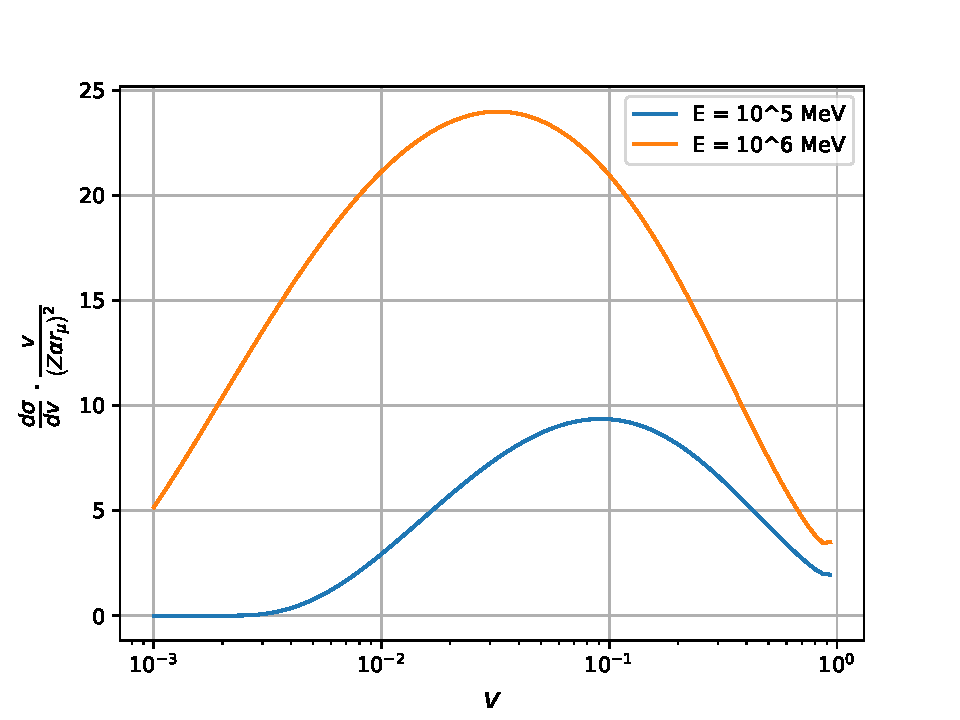
\includegraphics[height=0.8\textheight, trim=0cm 0.2cm 0cm 1cm,clip=true]{plots/mupair_crosssection.pdf}
    \caption*{Differential cross section in $v$ for two different muon energies. Propagation in standard rock.}
    \label{fig:1}
\end{figure}

\end{frame}


\begin{frame}
\vspace{-5mm}
  \begin{columns}
    \column{0.4\textwidth}
Continous energy loss per distance
\begin{align*}
  - \left\langle \frac{\mathrm{d}E}{\mathrm{d}x} \right\rangle &= E \frac{N_\text{A}}{A} \int_{v_\text{min}}^{v_\text{cut}} v \frac{\mathrm{d}\sigma}{\mathrm{d}v} \mathrm{d}v
\intertext{%
with}
v_\text{min} &= \frac{2 m_\mu}{E}, \\
v_\text{max} &= 1 - \frac{m_\mu}{E}. \\
\end{align*}
    \column{0.6\textwidth}
\begin{figure}
    \centering
    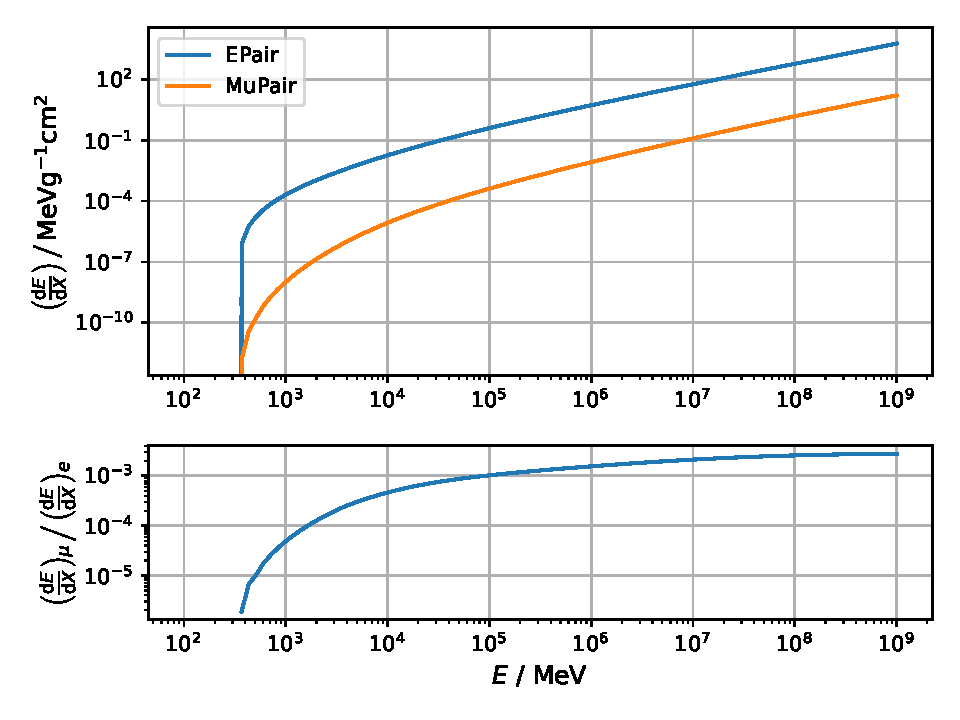
\includegraphics[height=0.85\textheight, trim=0.5cm 0.5cm 0.4cm 0cm, clip=true]{plots/mupair_compare.pdf}
    \caption*{Comparion of $e$-pair and $\mu$-pair production, only continous losses (i.e.\ $v_\text{cut} = v_\text{max}$).}
    \label{fig:2}
\end{figure}
  \end{columns}

\end{frame}

\begin{frame}
\vspace{-5mm}
  \begin{columns}



    \column{0.62\textwidth}
\begin{figure}
    \centering
    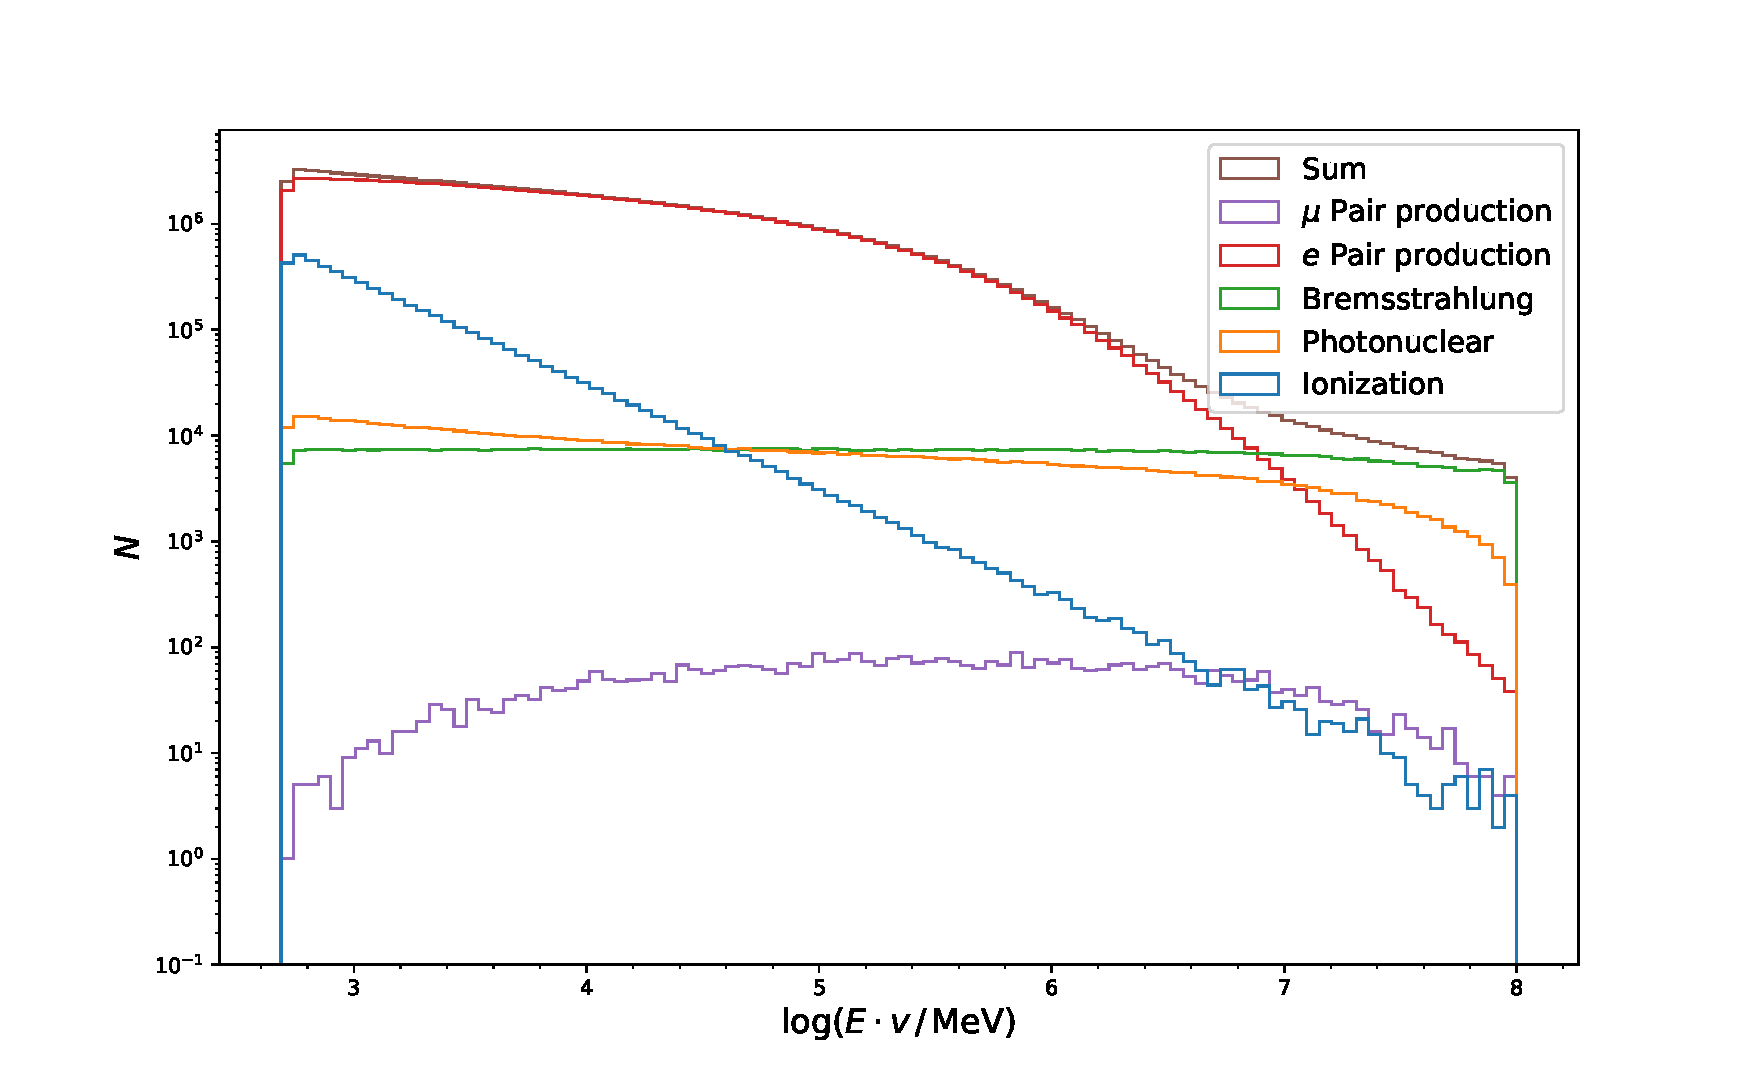
\includegraphics[height=0.8\textheight, trim=1.9cm 0.5cm 2.9cm 2cm, clip=true]{plots/mupair_secondaries.pdf}

    \label{fig:2}
\end{figure}

    \column{0.32\textwidth}
    \small
    \begin{table}
      \centering
      \begin{tabular}{c c c}
        \toprule
        $\text{process}$ & $N \,/\, N_\text{ges}$ & $E \,/\, E_\text{ges}$ \\
        \midrule
        $e$ pairp. & \num{0.94} & \num{0.94} \\
        Ioniz. & \num{4e-2} & \num{5e-2} \\
        Brems. & \num{1e-2} & \num{7e-3} \\
        Photon. & \num{8e-3} & \num{6e-3} \\
        $\mu$ pairp. & \num{6e-5} & \num{5e-5} \\
        \bottomrule 
      \end{tabular}
    \end{table}

  \end{columns}
  \small
    \vspace{5mm}
    Stochastic losses, standard rock, \num{e6} muons with $E = \SI{e8}{\mega\electronvolt}$, $e_\text{cut} = \SI{500}{\mega\electronvolt}$, $v_\text{cut} = \num{5e-2}$.
\end{frame}

\begin{frame}
\vspace{-3mm}

\begin{figure}
    \centering
    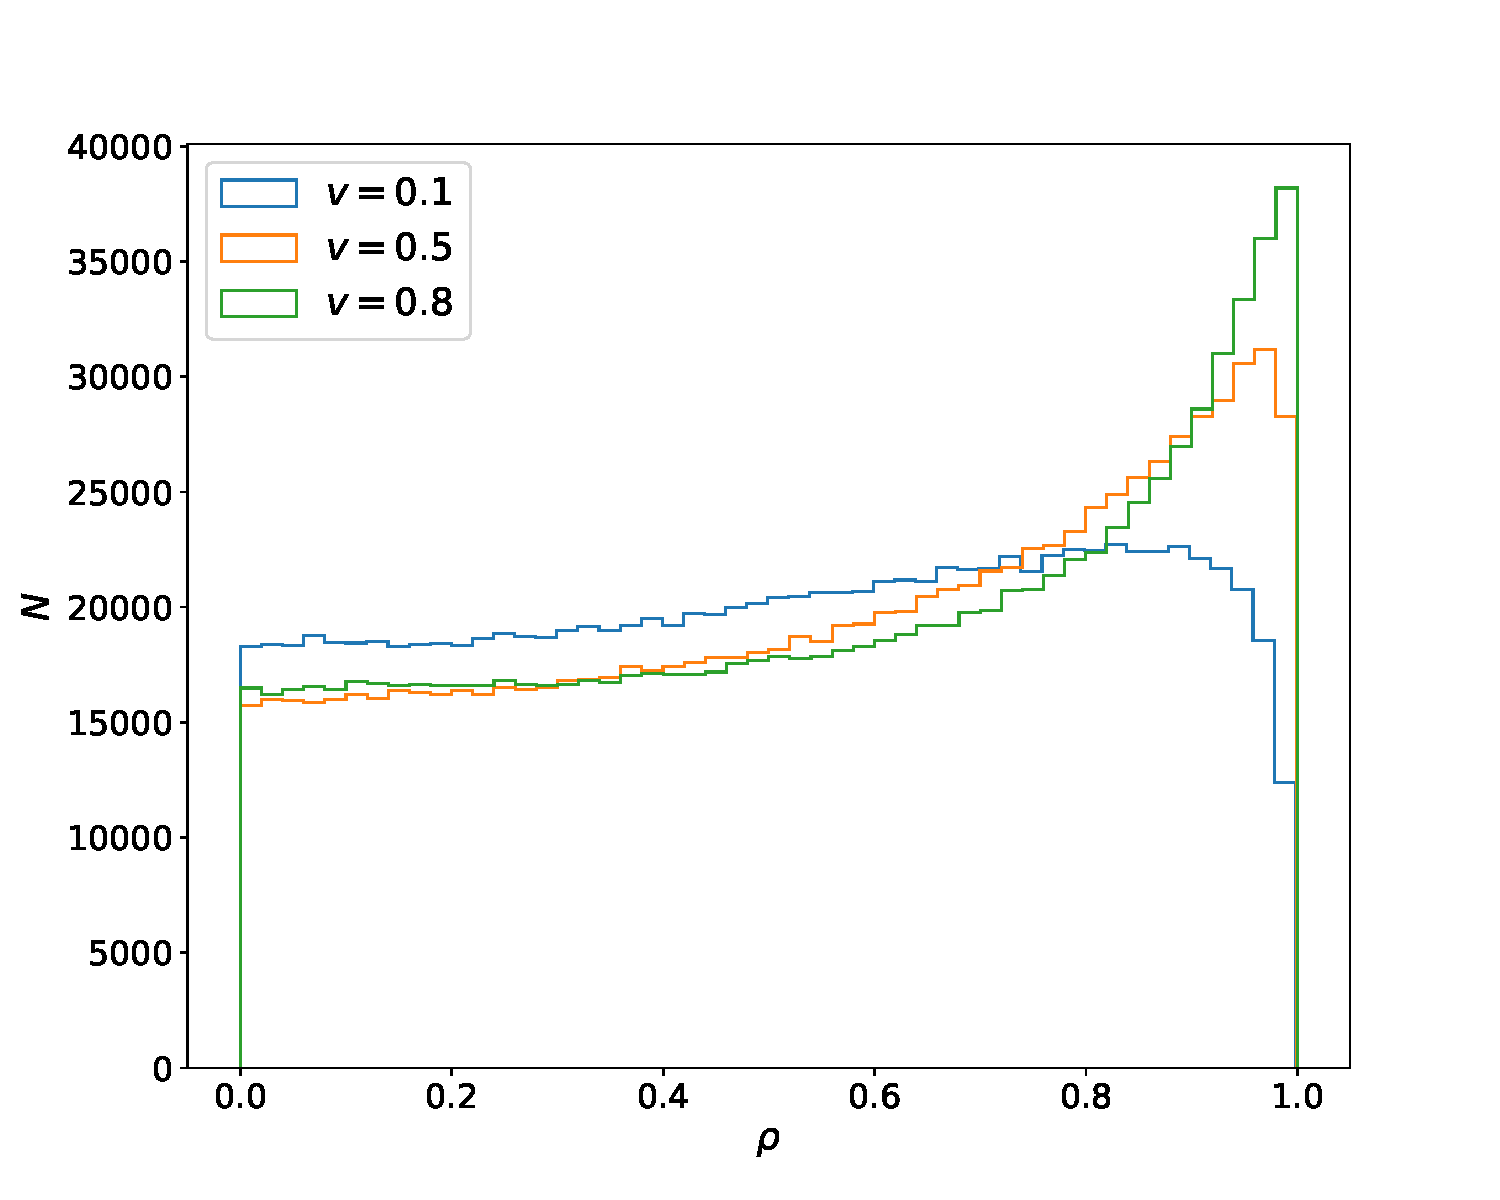
\includegraphics[height=0.9\textheight, trim=0.3cm 0.5cm 0.3cm 2cm,clip=true]{plots/plot_01.pdf}
    \caption*{Sampling of $\rho$ for muons with $E = \SI{1e6}{\mega\electronvolt}$ and different $v$ in standard rock.}
    \label{fig:1}
\end{figure}

\end{frame}

%%% Weak interaction %%%

\begin{frame}{Weak interaction}
  \begin{columns}
    \column{0.5\textwidth}
    \begin{center}
      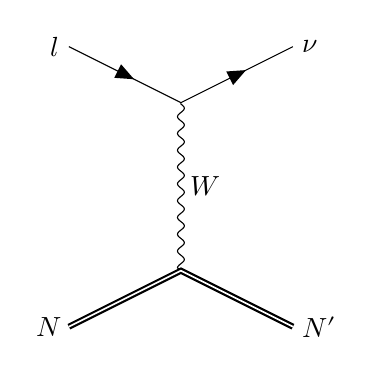
\begin{tikzpicture}
      \centering
       % Sizes
       \pgfmathsetmacro{\len}{0.05cm}
       \pgfmathsetmacro{\halflen}{\len/4}
       \pgfmathsetmacro{\vertexsize}{\len/20}
       \begin{feynman}
           % vertices
           \vertex (a) at (-1*\len, 0.5*\len);
           \vertex (b) at (0, 0);
           \vertex (c) at (1*\len, 0.5*\len);
           \vertex (d) at (0, -1.5*\len);
           \vertex (e) at (-1*\len, -2*\len);
           \vertex (f) at (1*\len, -2*\len);
     
           % draw diagram
           \diagram* {
             (a) -- [fermion] (b) -- [fermion] (c),
             (b) -- [boson, edge label=\(W\)] (d),

           };
           \draw[thick, double] (e) -- (d) -- (f);
     
           % labels
           \node[left] at (a) {$l$};
           \node[right] at (c) {$\nu$};
           %\node[right] at (f1) {$\mu^+$};
           %\node[right] at (f2) {$\mu^-$};
           \node[left] at (e) {$N$};
           \node[right] at (f) {$N'$};
      \end{feynman}
    \end{tikzpicture}
  \end{center}
  \column{0.5\textwidth}
    \begin{itemize}
      \item Highly suppressed process
      \item Similarities with "lollipop" signature in $\tau$-events
      \item Crossing symmetry\footnotemark:
      \begin{align*}
        \mathrm{d}\sigma\left( \mu Z \rightarrow \nu_\mu Z \right) = \frac{1}{2} \mathrm{d}\sigma\left( \nu_\mu Z \rightarrow \mu Z \right)
      \end{align*}
    \end{itemize}

  \end{columns}
  \footnotetext{Sandrock, Alexander: Higher-order corrections to the energy loss cross sections of high-energy muons, 2018, pp. 38-40}
\end{frame}

%%% Future %%%

\begin{frame}{Future: Physical improvements in PROPOSAL}
      \begin{itemize}
        \setlength\itemsep{0.5em}
        \item Improvement of electron propagation
        \item Propagation of high-energy photons
        \item Deflection of particles in magnetic fields
        \item Propagation through media with non-homogenous density
      \end{itemize}
\end{frame}


\begin{frame}[t]
  \vspace{-5mm}
  \begin{minipage}[t][0.8\textheight][t]{\textwidth}
      \begin{columns}
    \column{0.5\textwidth}
      \begin{figure}
          \centering
          
\includegraphics[width=0.6\linewidth]{plots/github.pdf}
           \captionsetup{format=myformat}
          \caption*{https://github.com/tudo-\\astroparticlephysics/PROPOSAL}
      \end{figure}
    \column{0.5\textwidth}
      \begin{figure}
          \centering
          
\includegraphics[width=0.6\linewidth]{plots/arxiv.pdf}
          \captionsetup{format=myformat}
          \caption*{https://arxiv.org/abs/1809.07740 \\ \phantom{astroparticlephysics/PROPOSAL}}
      \end{figure}
  \end{columns}
  \end{minipage}
  \vfill
  \begin{minipage}{\textwidth}
      \smaller
      \begin{center}
      PROPOSAL may be modified and distrubuted under terms of a modified LGPL license.\\More information on our GitHub page.
      \end{center}
  \end{minipage}
\end{frame}
\end{document}
